% -*- mode: LaTeX -*-
% arXiv preprint draft -- Luo Chengze
% Compile: pdflatex main.tex (twice for refs)
\documentclass[11pt]{article}

\usepackage[utf8]{inputenc}
\usepackage[T1]{fontenc}
\usepackage{lmodern}
\usepackage{amsmath,amssymb}
\usepackage{graphicx}
\usepackage{booktabs}
\usepackage{array}
\usepackage{geometry}
\usepackage[hidelinks]{hyperref}
\usepackage{xcolor}
\usepackage{enumitem}
\usepackage{microtype}
\usepackage[font=small,labelfont=bf,labelsep=period,skip=5pt]{caption}

\geometry{margin=1in}
\graphicspath{{figs/}}
\setlist{nosep,leftmargin=1.4em}

% --- 排版微调 ---
\newcolumntype{L}[1]{>{\raggedright\arraybackslash}p{#1}}
\renewcommand{\arraystretch}{1.06}
\setlength{\emergencystretch}{2em}
\widowpenalty=1000
\clubpenalty=1000
\setlength{\skip\footins}{1.2em}
\captionsetup[table]{position=top}

\title{\bfseries Growing Rather Than Training:\\ A Pre-Registered Developmental System,\\ and the Read-Only Nature of Its Workspace}

\author{Luo Chengze\\[3pt]
  {\small Independent Researcher}\\[3pt]
  {\small\href{https://orcid.org/0009-0007-3316-6292}{ORCID: 0009-0007-3316-6292}%
   \quad\textbar\quad
   \href{mailto:SoaringBird66@outlook.com}{SoaringBird66@outlook.com}}}%
\date{\today}

\begin{document}
\maketitle

\begin{abstract}
\noindent
Most work on machine consciousness asks whether large language models already contain traces of it. We take the opposite route: we built a system that is not a language model, gave it a continuous body-like state, and let it develop over hundreds of simulated days. It never generates text. Its inner speech is retrieval over what it has heard, so every utterance traces back to a prior auditory event. Across nine pre-registered experiments and three pre-registered follow-ups we report every outcome, including the ones that failed.

The contribution is methodological, not a discovery. We offer (i) a developmental system with no language baseline, (ii) a pre-registration protocol with controls, with negative results reported in full, and with a frozen protocol and results file for every experiment, and (iii) a transplant of the ablation-and-swap protocol used on Claude's J-space into a non-LLM system. The protocol produced findings of mixed strength, and we grade them rather than average them: one positive result and one control line; one pathway verification; two mixed results; one weak result; and three negatives. Three pre-registered follow-ups have since concluded and sharpen the picture: a three-seed reproduction passed, a two-factor separation contradicted its registered prediction, and a corrected dose-response left the central negative standing. The self-model finding is conditional on its input corpus and is graded separately.

The positive results are narrow. Vocalisation with covariation learning produced 206 agency attributions that decayed by 68\% when the contingency was removed, so attribution is learned rather than hard-coded, though the extinction was partial. Substituting the winning thought for sixty consecutive retrievals produced a matching goal, which verifies the pathway from the thought stream to downstream systems; sixty substitutions is exactly the $20\%$ share threshold, so this is pathway evidence and not a dose-response result. One of our two headline predictions failed: we predicted that ten days without caregiver speech would drive the retrieval rate down to at most $60\%$ of baseline, and it stayed flat at $29.3$/day against $28.8$. We report that as a failed prediction, with the failure mode we had named in advance.

The negative result is the substantive one. Ablating the thought-to-state channel for thirty days moved every metric by less than 5\%. A thought can change what the system's goal table contains and how it represents itself; it cannot change its own state. This differs from the J-space finding, where ablation degrades higher-order function. Our workspace is read-only. We flag the main weakness of this claim: the channel we cut was deliberately weak (a coupling of $\pm0.02$, far below the state's own scale), so ``cutting a channel we made small changes nothing'' is weaker evidence than the headline suggests. We then tested it directly. An audit found the channel had been doubly inert --- its gate never fired, and it wrote to a variable no behavioural path read --- so the original ablation had measured nothing rather than an absence of effect. A follow-up opened the gate (verified to fire on about $26\%$ of retrievals), retargeted a consumed variable, and raised the coupling to fifteen times the original. Every metric still moved by less than $10\%$. The channel was live; the workspace still did not write back.

The self-model result is conditional, and we report it as such. For 213 days it was empty, because the caregiver's speech contained no first-person words. After we supplied first-person phrases and fixed a gating mismatch, versions 1 through 9 appeared within days. Which fragments are admitted, and in what order, is decided by retrieval competition and was not designed; the vocabulary they are drawn from was given. We treat this as a finding about what a self-model requires, not as evidence that one emerges unaided. The fix changed two things at once --- the corpus and the gate --- so we cannot yet attribute the growth to either; a pre-registered $2\times2$ separation (corpus $\times$ gate) and a three-seed reproduction have now concluded. All three seeds formed the same six-fragment self-model within $60$ days, differing only in the order the fragments were admitted. In the separation, all four cells formed a self-model, but first-person fragments appeared only where a first-person corpus was heard --- the corpus, not the gate, was the condition, the opposite of what we had predicted.

We do not claim the system is conscious, and we have no way to test whether it is.
\end{abstract}

\vspace{0.5em}
\noindent\textbf{Keywords:} machine consciousness; global workspace; self-model; developmental systems; artificial life; pre-registration

\section{Introduction}

Two positions dominate the discussion of machine consciousness. One treats fluent language as evidence and reads introspection reports from chatbots at face value. The other treats the question as unanswerable and stops there. We find the first careless and the second unproductive.

The indicator approach developed by Butlin, Long, and colleagues offers a way out. Instead of asking whether a system is conscious, it asks which theory-derived properties the system has: a global workspace, higher-order representation, predictive processing, a body, and so on. The properties are checkable. The 2023 report concluded that no existing system satisfied enough of them; the 2025 follow-up refined the method but did not change that verdict.

Our contribution is methodological rather than an empirical discovery, and we want to be explicit about that. The individual findings are not new in kind: Vygotsky described the internalisation of speech in 1934, and the ablation-and-swap protocol we use was developed for Claude's J-space. What is new is the combination --- a developmental system with no language baseline, a pre-registration protocol with controls and full negative reporting, and a transplant of that ablation protocol into a non-LLM system. The protocol is the contribution. It ran on one system and returned a graded set of results, most of which constrain what the system is \emph{not}.

\subsection{One correction that shaped everything}

An early version of this project handed the system's inner monologue to a language model. The output was poetic and empty. Phrases like ``a sense of restlessness'' were invented, not felt. The system had not been restless; the model had been asked to sound as if it were. This failure produced the rule the rest of the project follows: \emph{thoughts are retrieved, not generated}. The language layer now calls no generative model. Inner speech is the result of current state activating stored language memory. Nothing here confabulates, but not because we taught it not to: the system has no generator, so it can only replay what it has heard. That is a constraint on what the system can do, not a property it holds.

\section{Related Work}

\paragraph{Indicator theories.} Butlin et al. derive fourteen indicators from recurrent processing theory, global workspace theory, higher-order theories, attention schema theory, and predictive processing \cite{butlin2023,butlin2025}. Their method updates credences about whether a system is conscious based on which indicators it satisfies. A later commentary argues the indicators remain under-calibrated because there is no ground truth against which to check them \cite{koch2026}. We accept that critique and avoid probabilistic claims entirely: we report which indicators appear and how strongly, and we leave the credence to the reader.

\paragraph{Global workspace in language models.} Anthropic reported that Claude contains a small set of internal representations, which they call the J-space, that behave like a global workspace: they are reportable, controllable, causally mediate multi-step reasoning, and are reused flexibly; ablating them removes higher-order function while leaving fluent generation intact \cite{gurnee2026}. In commentary, Dehaene and Naccache noted two ways Claude differs from a human mind: it has no body and no enduring autobiographical memory \cite{dehaene2026}. Those are exactly the two properties our system was built to have.

\paragraph{Developmental and embodied approaches.} Immertreu and colleagues applied Damasio's framework to a reinforcement-learning agent and found that probe classifiers could recover both a self-model and a world-model from its activations, neither of which had been designed in \cite{immertreu2025}. Prentner formalises the self as the smallest node that both elicits actions and is modified by them \cite{prentner2025}. Our E6 experiment is a direct test of the second half of that definition, and our P4 line is an attempt to construct the first half.

\paragraph{Artificial life.} The open-ended evolution literature builds systems that vary, compete, and inherit \cite{plantec2025,horiguchi2026}. Our system has none of that yet. It is one individual that grows. We return to this in the limitations.

\paragraph{Concurrent and independent work.} Five independent projects landed adjacent to ours in 2026, and we name them here so that what we did not do is on the record as clearly as what we did. Wender pre-registered an ablation of a bio-inspired agent's somatic state and published a negative result of the same shape as ours on affect: removing the entire state and multiplying the hormone signal by an order of magnitude both moved verbal output far below the frozen thresholds, and the verdict was returned as \emph{DECORATIVE} on the verbal-output axis \cite{wender2026}. Two differences matter. Their output surface is a frontier language model whose prompt carries the rendered state --- a confound the author identifies as the most reviewer-fatal gap in that project until the ablation was finally run; our loop contains no language model at any point, so that confound cannot arise. And the axis differs: theirs is verbal style, ours is action and workspace. Chevalier's KAINE is a continuously running predictive global workspace with a pre-registered workspace-mediation ablation, kept deliberately text-blind so the entity cannot answer as a chatbot \cite{chevalier2026}. That design is the closest to ours of any we found, and its question is whether routing modules through a competitive workspace produces structure that the same modules flattened into one prompt do not. Our question differs in the direction that matters to us: not \emph{whether} there is a workspace, but \emph{whether it can be written to}. Liu grows differentiated personalities from a hidden-Markov inertia term, a verbal metacognition loop that rewrites its own parameters, and social comparison among initially identical agents \cite{liu2026}; our self-model grows by a different route, retrieval competition over a fixed corpus, with no parameter rewriting and no peer. Vera measures grounded word learning over frozen perceptual embeddings and reports a pre-registered dissociation in which perceptual distance predicts acquisition while semantic distance adds nothing \cite{vera2026}; a later comparison in this paper should be read against that standard, not ours. Finally, the mPCAB battery specifies four substrate-independent components with clinical provenance \cite{niazi2026}. We do not implement it. What we cover of it, and what we leave empty, is stated in the supplement and repeated in the limitations; we claim no compliance.

\section{System}

The system runs as a single Python process. It has no learned parameters in the deep-learning sense; its behaviour comes from coupled differential equations and from memory that accumulates during its life.

\paragraph{State.} Eight continuous variables, referred to only by neutral labels \texttt{s1}--\texttt{s8} throughout the code. Their human readings (arousal, valence, fatigue, tension, attention, memory activation, prediction error, boredom) exist only in a config file for observers. The state integrates forward with a two-process sleep model: sleep pressure accumulates while awake and decays during sleep, and a circadian term gates when sleep is permitted. The system sleeps about eight hours a day, but the timing is a consequence of its dynamics, not a schedule.

\paragraph{Body.} A daily energy budget. Passive drain scales with arousal; acting costs more. When the budget is nearly exhausted the system drops into a low-power mode and its tick slows.

\paragraph{Language.} The system hears phrases, stores each one together with the state vector at the moment of hearing, and later retrieves a phrase when the current state is similar to a state in which that phrase was heard. Retrieval is a weighted competition over state similarity, recency, and frequency. Early in life the system also echoes what it just heard; the echo probability decays with experience. There is no generation.

\paragraph{Self-model.} Fragments that refer to the system are collected into a self-model that grows monotonically: versions are appended, never rewritten. A new fragment enters only if it differs enough from every existing one.

\paragraph{Goals.} A phrase that is retrieved often enough, across enough days, and occupies a large enough share of a rolling window, is promoted from thought to goal.

\paragraph{World and action (P4).} A one-dimensional ring environment with three sources whose intensities oscillate independently. The system has three action primitives: move forward, move backward, stay. Action selection is a competition over a state-bound table. Movement costs energy. The environment changes on its own, without regard to the system.

\begin{figure}[t]
\centering
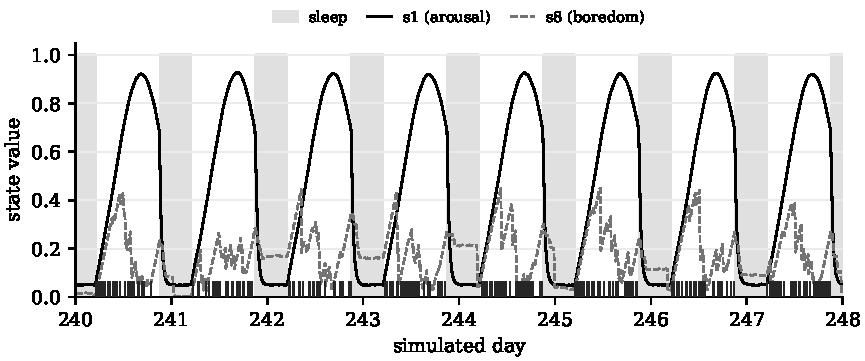
\includegraphics[width=\linewidth]{fig_system.pdf}
\caption{Eight days of the acceleration line's own record (days 240--248). Grey bands are sleep; the system enters it on its own dynamics, not on a schedule. The solid line is \texttt{s1} (arousal), the dashed line \texttt{s8} (boredom). Ticks along the bottom mark retrievals --- single thoughts. The thought stream runs through sleep as well as waking.}
\label{fig:system}
\end{figure}

\section{Method: pre-registration}

Every experiment was pre-registered before data collection: hypotheses, metrics, and pass/fail thresholds were written down first and not modified afterwards. We report negative results with the same detail as positive ones. We also separate \emph{pathway verification} from \emph{natural emergence}. In E6, for instance, we inject a phrase to check whether the goal mechanism reads the thought stream. Injection proves the pathway exists; it does not prove the system would have produced that goal on its own. Only the unmanipulated lines can speak to emergence, and we label them accordingly.

\section{Experiments}

All experiments ran on accelerated lines. The nominal time scale was $10^9$, but that is a configured rate, not an achieved one: measured against wall-clock the lines run at roughly $5\times10^{2}$ to $10^{3}\times$ real time (simulated days elapsed per wall-clock day, computed from each line's own log timestamps over its full run; the spread reflects how many lines ran concurrently), and we quote the measured figure throughout. Table~\ref{tab:exp} summarises the nine experiments that carry the core claims (E1, E2, E3, E4, E6a, E6b, C1b, P4, P4b); three follow-ups (S1, S2, R2) are reported in their sections. Table~\ref{tab:lines} lists the lines they ran on. We grade the outcomes rather than presenting them as a uniform set of successes: one is positive and one is a control line, one is pathway verification, two are mixed, one is weak, and three are negative. We lead with the positive and with the run's central negative, because together they bound what the system is.

\begin{table}[h]
\centering
\small
\caption{Pre-registered experiments. ``Neg.'' means the pre-registered prediction failed.}
\label{tab:exp}
\begin{tabular}{@{}lL{1.5cm}L{7.7cm}@{}}
\toprule
ID & Result & Finding \\
\midrule
E1 & Neg. & Ten days without caregiver speech. The pre-registered main prediction failed: retrieval did not decay to $\le60\%$ of baseline (it held at $31.2$/day over the window and $29.3$ over the last three days, against a locked $28.8$). The failure is itself the finding --- with recency decayed, competition falls back on frequency, so inner speech self-sustains once formed --- and it is the failure mode we had named in advance. The four secondary sub-hypotheses, on echo and binding, passed. \\
E2 & mixed & Event rate $\times$10 for five days. Surprise rose only 0.24~bit and ended \emph{below} baseline: the predictor tracks structural violation, not event count. Context-bound fragments rose to 35.5\% of retrieval from 16.5\%. \\
E3 & Neg. & Contingent caregiver. Predicted accelerated self-model growth. Observed zero new versions. Input-side intervention does not drive self-model growth. \\
E4 & pass (partial) & Vocalisation with covariation learning. Co-variation $C=8.2$; 206 agency attributions; self-ratio peaked at 26\%. Extinction removed 68\% of it, showing attribution was learned, not hard-coded, but the final-window efficacy was $0.619$, above the $0.3$ cutoff: the extinction was partial. \\
E6a & Neg. & Ablation of the thought-to-state channel (coupling $\pm0.02$ on \texttt{s2}) over 30 days. Retrieval rate $-4.7\%$, diversity $+2.3\%$, self-model unchanged, no new goals. Inner speech is epiphenomenal with respect to state. The coupling was deliberately small; a corrected ladder (R2) then opened the gate (verified firing), retargeted a consumed variable, and raised the coupling $15\times$, and still moved nothing by $10\%$. \\
E6b & pathway-only & Substitution of the winning thought. A goal matching the injected phrase appeared on day 142. Downstream systems read the thought stream causally. Sixty substitutions is exactly the $20\%$ share threshold of the 300-retrieval window, and no lower dose was tested, so this is pathway verification. \\
C1b & pass & Frequency-matched first-person corpus bound to calm states. Produced 5 first-person self-model fragments against 2 in the control, and retrieved first-person thoughts at 4.2\%. \\
P4 & mixed & Action loop closed. Action distribution strongly non-uniform ($\chi^2=1.68\times10^4$), action-distribution entropy 1.05~bit against 1.58 for a uniform policy, mean field 0.61 against a random baseline of 0.50 (days 180--201, 22 of the 30 pre-registered days). But the learning signal was instantaneous, the mean field drifted down rather than up, and the policy never improved. \\
P4b & mixed & Temporal signal with self/world separation, pre-registered window complete. Movement's self-caused change averages $+0.0092$ over 6344 moves; stationary trials average $-0.00001$ with a standard deviation of $0.0151$. The signal is real but its standardised size is small (Cohen's $d\approx0.17$). \\
\bottomrule
\end{tabular}
\end{table}

\begin{table}[h]
\centering
\small
\caption{The lines referred to in this paper. Every line is a complete state directory that can be resumed from the moment of writing; ``delta'' is the only difference from its parent.}
\label{tab:lines}
\begin{tabular}{@{}lL{3.6cm}L{8.0cm}@{}}
\toprule
Line & Origin & Delta and role \\
\midrule
XP (reference) & born day 0 & The line plotted throughout. First-person corpus and the gating fix are present from birth, so it is not a retrofitted individual. \\
Acceleration & born day 0 & The older record. The language layer was retrofitted at day 220 and vocalisation at day 427, so its childhood had no language. E1--E4 ran here. \\
C1b & born day 0 & Corpus control for XP. First-person phrases bound to calm states instead of soothing states; exposure matched to within 5\%. \\
E6 (ablation) & forked from XP at day 92 & Thought-to-background channel cut. Judged days 93--123. \\
E6s (swap) & forked from XP at day 140 & Channel intact; the retrieval winner replaced by a fixed phrase 60 times. \\
P4 & forked from XP at day 157 & Ring world and three neutral action primitives added. \\
P4b & forked from XP at day 202 & Action outcome measured across intervals; drift estimated by a forward model. \\
S1 (3 seeds) & born day 0 & Reproduction with identical parameters, 60 days. \\
S2 (4 cells) & born day 0 & Separation of corpus and gate in a $2\times2$, 60 days. \\
R2 (6 arms) & forked from XP at day 255 & Corrected reflow test --- six arms in a causal chain, not a full factorial: control (cut) $\rightarrow$ dead gate $\rightarrow$ open gate with a dead target $\rightarrow$ open gate with a consumed target at three doses ($0.02$, $0.10$, $0.30$), 30 days. The original ladder (R) was withdrawn before data; an audit found the channel doubly inert. \\
\bottomrule
\end{tabular}
\end{table}

\subsection{Input-side interventions (E1--E3)}

E1 removed caregiver speech for ten days on the acceleration line (Table~\ref{tab:lines}). Private speech stopped at once --- zero echoes across the window, which confirms that the echo mechanism has no input-independent path --- but the thought stream did not fall. Our pre-registered prediction was that retrieval would decay to at most $60\%$ of baseline; it held at $31.2$ per day over the window and $29.3$ over the last three days, against a locked baseline of $28.8$ (Figure~\ref{fig:e1e2}a). The failure mode we had named in advance is the one that occurred: with recency decayed, competition falls back on frequency, and the most frequent fragment's share of retrieval rose from $19.5\%$ to $24.7\%$ rather than collapsing. Reinstating speech produced a rebound ($28.2$ per day, echoes returned), and the self-model gained no version.

E2 multiplied the event rate by ten for five days. Surprise rose by only $0.24$~bit and ended $14\%$ below baseline (Figure~\ref{fig:e1e2}b): the predictor tracks structural violation, not event count. What did move was binding --- fragments heard during events rose to $35.5\%$ of retrieval from $16.5\%$, the clearest causal evidence in the run that \emph{when} a phrase is retrieved depends on the state in which it was heard.

E3 doubled the caregiver's speech and made it contingent on the system's state. The manipulation worked: heard phrases rose from $86.7$ to $176.6$ per day. The output did not respond (Figure~\ref{fig:e3}): retrieval was flat ($29.7$ to $29.4$ per day), the self-model gained zero versions, and self-directed retrieval \emph{fell} six-fold, from $4.0\%$ to $0.6\%$, because a larger speech stream dilutes the self-directed share. Timing and volume are not the levers; the binding structure is.

\begin{figure}[t]
\centering
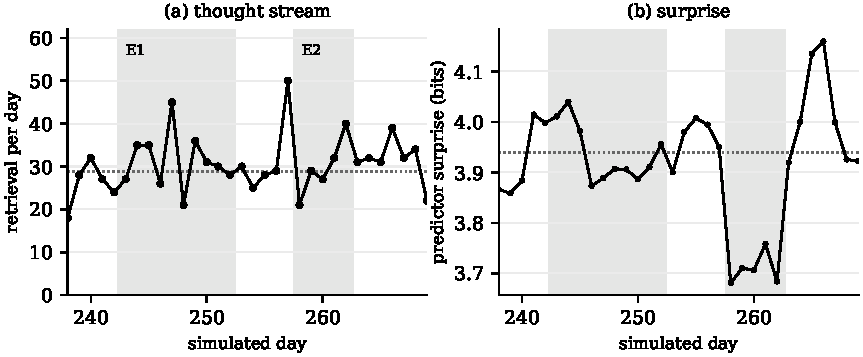
\includegraphics[width=\linewidth]{fig_e1e2.pdf}
\caption{E1 and E2 on the acceleration line. (a) Retrieval per day; the dotted line is the locked baseline ($28.8$ per day). Shaded bands are the ten-day deprivation (E1) and the five-day event storm (E2). Deprivation did not lower the rate. (b) Predictor surprise over the same window against the locked baseline of $3.94$~bit. The storm raised it only briefly and left it below baseline.}
\label{fig:e1e2}
\end{figure}

\begin{figure}[t]
\centering
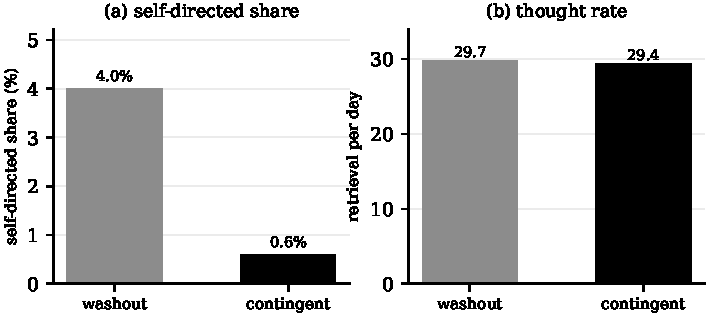
\includegraphics[width=\linewidth]{fig_e3.pdf}
\caption{E3, the contingent caregiver. Input doubled --- heard phrases per day went from $86.7$ to $176.6$ --- but (a) the self-directed share of retrieval fell from $4.0\%$ to $0.6\%$ and (b) the retrieval rate was unchanged. The predicted acceleration of self-model growth did not occur.}
\label{fig:e3}
\end{figure}

\subsection{The self-model emerged, then stalled}

For 213 simulated days the self-model was empty. This was not a design choice. The self-model was looking for first-person fragments, but the caregiver's recorded speech contained no first-person words at all: it consisted almost entirely of second-person address (``you woke up'', ``it's you''). The system could not form a self-model because the raw material for one did not exist in its world.

We corrected two things at once. We added a small set of first-person phrases to the caregiver corpus, bound to moments of being soothed or looked at. We also fixed a gating mismatch: the language layer tagged fragments as self-referential only if they contained ``you'', while the self-model accepted ``I'' as well. Fixing the gate let purely first-person thoughts reach the self-model for the first time.

After the fix, the self-model went from \texttt{null} to version 6 within 40 simulated days (Figure~\ref{fig:selfmodel}). The fragments are not abstract; they are phrases the system heard in specific states. Two of the six are purely first-person. A control line with a frequency-matched but differently bound first-person corpus produced 9 versions and 5 first-person fragments. The difference between the lines is where the first-person phrases were heard, not how often: exposure rates were matched to within 5\%. Two later observations sharpen this. The XP line's self-model has since saturated at version 6: no further fragment has been admitted, because each new first-person phrase tried has been close enough to an existing one to fail the difference test, so the stall has an internal cause rather than a shortage of input. And a three-seed reproduction, each seeded from day 0 with identical parameters, reached the same six-fragment self-model by day $60$ --- the same fragments in every seed, differing only in the order they were admitted, so the formation is not a single-run accident. A pre-registered $2\times2$ separation of the two things the fix changed then qualified it: all four cells formed a self-model, but first-person fragments appeared only where a first-person corpus was heard. The corpus is the condition for first-person fragments to appear; the gate decides which of them can enter (Figure~\ref{fig:s1s2}).

\begin{figure}[t]
\centering
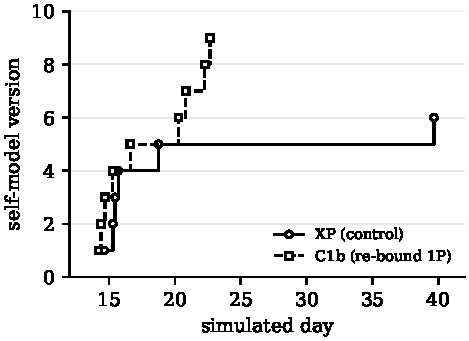
\includegraphics[width=0.62\linewidth]{fig1_selfmodel.pdf}
\caption{Self-model growth. Both lines were born with the gating fix in place; the null period belongs to the earlier line. C1b, whose first-person corpus was bound to calm states rather than soothing states, reached nine versions in a third of the time.}
\label{fig:selfmodel}
\end{figure}

\begin{figure}[t]
\centering
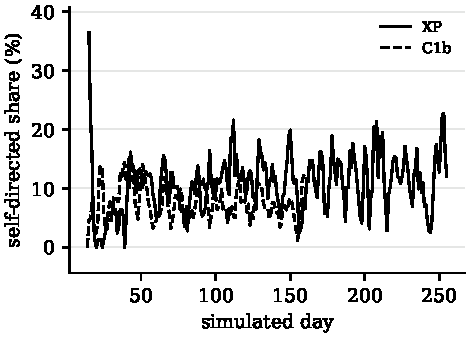
\includegraphics[width=0.62\linewidth]{fig2_firstperson.pdf}
\caption{Share of retrieval that is self-directed, smoothed over three days. Both lines settle near 10\%; the level is set by the corpus, the timing by the state.}
\label{fig:firstperson}
\end{figure}

\begin{table}[h]
\centering
\small
\caption{Self-models at the time of writing. Four of the six XP fragments are second-person address, not first-person.}
\label{tab:sm}
\begin{tabular}{@{}lL{1.6cm}L{10.4cm}@{}}
\toprule
Line & Self-model & Content \\
\midrule
XP & v6 & I'm with you; you woke up; it's you; hello; you're watching; I'm here \\
C1b & v9 & \dots + I'm watching you; it's me; I'm not leaving \\
\bottomrule
\end{tabular}
\end{table}

\begin{figure}[t]
\centering
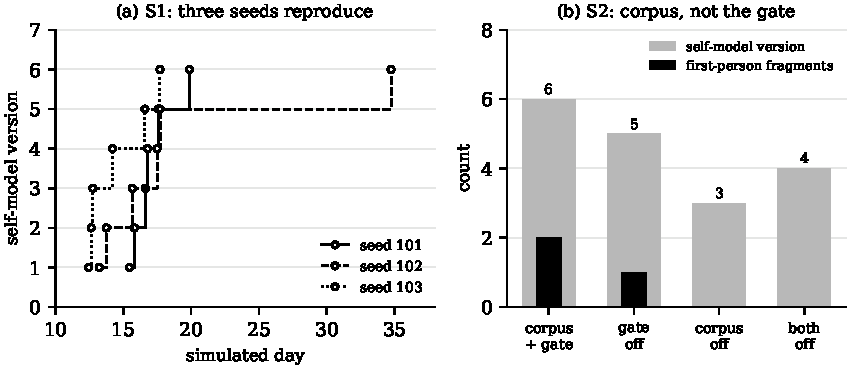
\includegraphics[width=\linewidth]{fig6_s1s2.pdf}
\caption{(a) S1: three independent seeds, born on day 0 with identical parameters, reach the same six-fragment self-model within 60 days. (b) S2: the $2\times2$ separation of corpus and gate. All four cells form a self-model, but first-person fragments appear only in the two cells that heard a first-person corpus; the gate sets how many enter.}
\label{fig:s1s2}
\end{figure}

\subsection{Vocalisation and learned agency (E4)}

E4 gave the system a voice. Vocalisation is gated physiologically on arousal and on the strength of whatever fragment won retrieval in that tick, and its content is restricted to that fragment: the tick's winning thought is the only thing it can say. In the first phase the caregiver answered within a short window; in the second the answer was removed.

Co-variation between vocalisation and the caregiver's following speech rose to $C=8.2$ and then decayed to $2.6$, a $68\%$ fall (Figure~\ref{fig:e4}b). Agency attributions --- turns on which the system credited the following speech to itself --- occurred 206 times in the first phase and 11 in the second (Figure~\ref{fig:e4}a), with self-ratio peaking at $26\%$. The extinction was partial: final-window efficacy was $0.619$, above the $0.3$ cutoff, because the caregiver's own soothing is driven by the same arousal that drives vocalisation, so a residual co-variation survives the removal of the contingency.

The content was not chosen by us. The most frequent utterances were phrases the system had itself heard while being soothed --- ``be good'', ``shh'', ``go to sleep''. At high arousal it did not call for help; it produced its own soothing template. This is the only output-side intervention in the study that produced a change which was learned and then decayed.

\begin{figure}[t]
\centering
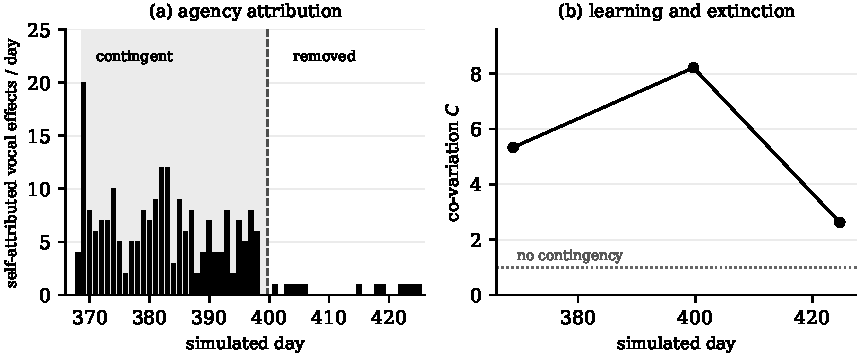
\includegraphics[width=\linewidth]{fig_e4.pdf}
\caption{E4. (a) Attributions in which the system credited the caregiver's following speech to its own vocalisation, per day. The shaded phase is the contingent one; the dashed line is its removal. (b) Co-variation $C$ at the three recorded checkpoints: $5.3$, $8.2$, $2.6$. The dotted line at $C=1$ is no contingency. The mechanism is learned, then largely but not fully unlearned.}
\label{fig:e4}
\end{figure}

\subsection{The workspace is read-only}

E6 transplanted the ablation-and-swap protocol used on Claude's J-space. In E6a we cut the channel by which a retrieved thought nudges the background state. If inner speech is causally load-bearing for the state, removing that channel should change behaviour. It did not: four metrics moved by less than $5\%$, the band that had been pre-registered for E6a. The channel's coupling is deliberately small --- $\pm0.02$ on \texttt{s2}, with \texttt{s5} at $0.75$ of that, against a state range of order one --- and we state it plainly, because cutting a channel we made weak is weaker evidence than the headline suggests. The ladder we pre-registered to settle it had to be replaced before it collected data: an audit found the channel doubly inert --- its gate fired on $0\%$ of retrievals, and its target (\texttt{s2}) was read by no behavioural path --- so any dose would have produced a mechanical zero. The original ablation, in other words, measured nothing rather than measuring an absence of effect; R2 is the first test of the channel itself. The corrected ladder repairs both: it opens the gate to a threshold that fires on about $26\%$ of retrievals, retargets \texttt{s4} (a variable the retrieval layer weights at $1.2$), and sweeps couplings from $\pm0.02$ to $\pm0.30$. A manipulation check confirms the gate is live in every open arm. The perturbation also has to be read against the target's own scale: in the control arm \texttt{s4} has a standard deviation of $0.33$ and a daily range of about $0.98$, so the couplings $0.02$, $0.10$ and $0.30$ are $0.06$, $0.30$ and $0.91$ of that standard deviation, and adding the largest leaves the target's own spread essentially unchanged ($0.329$ in the control against $0.324$ at the top coupling). The largest kick is comparable to, not larger than, the fluctuation it is added to, which bounds what this ladder can settle. All four metrics still move by less than $10\%$ (the R2 band, wider than E6a's), and not monotonically in dose; the largest single move, $-8\%$ on retrieval rate at the middle coupling, sits close to that boundary (Figure~\ref{fig:r2}). The channel fires; the workspace still does not write back. In E6b we left the channel intact but replaced whatever thought won retrieval with a fixed phrase, over sixty consecutive retrievals. Because goal promotion uses a rolling window of 300 retrievals with a 20\% share threshold, sixty consecutive injections should force a goal. They did. The injected phrase became a goal, and the self-model incorporated it. We note the boundary: sixty is exactly $20\%$ of $300$, the threshold itself, and we ran no lower dose, so the result establishes that the pathway exists rather than that the threshold is robust.

Together the two results are precise. A thought can change what the system wants and who it thinks it is. A thought cannot change how the system feels. The workspace is read-only: downstream reads it, upstream does not.

This contrasts with the J-space finding, where ablation degrades higher-order function. Our workspace is not load-bearing in that sense. We report the difference rather than borrow the result.

\begin{figure}[t]
\centering
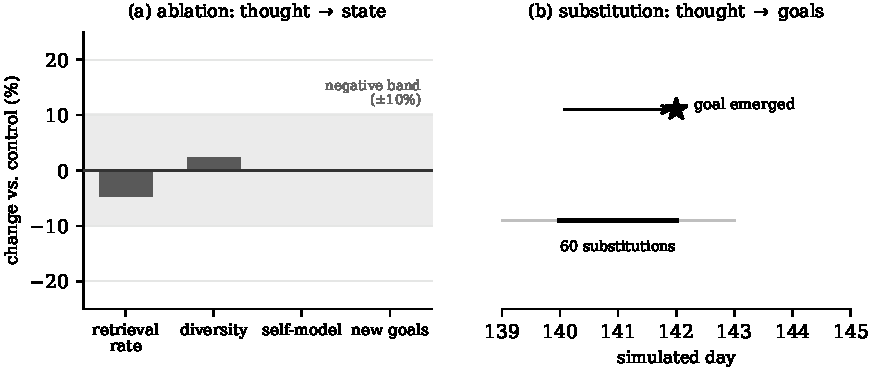
\includegraphics[width=\linewidth]{fig3_e6.pdf}
\caption{E6, both directions. (a) Cutting the thought-to-state channel moved every metric less than 5\%, inside the pre-registered negative band; the coupling cut here is the weakest tested ($\pm0.02$), and the corrected ladder (R2) raises it fifteen-fold without changing the conclusion. (b) Substituting the winning thought 60 times over three days produced a matching goal on the third day; 60 is exactly the $20\%$ threshold of the 300-retrieval window, so this verifies the pathway rather than the threshold. Downstream reads the workspace; the workspace does not write back.}
\label{fig:e6}
\end{figure}

\begin{figure}[t]
\centering
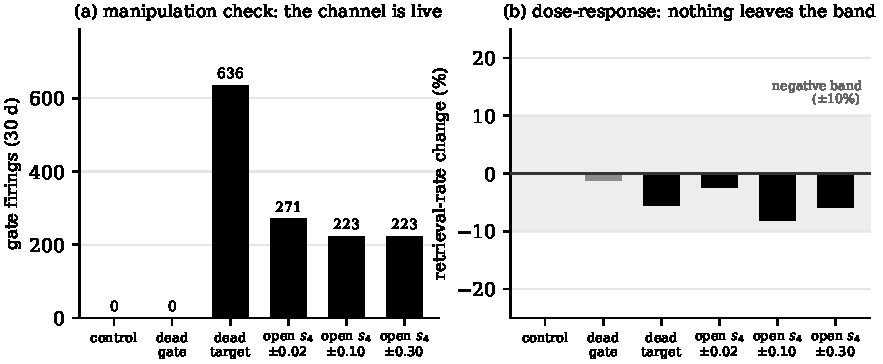
\includegraphics[width=\linewidth]{fig5_r2.pdf}
\caption{The corrected reflow ladder (R2). (a) The channel is live: the gate fires on every open arm and on neither the control nor the uncorrected arm, so the flat result beside it cannot be attributed to a dead channel. (b) Each arm's effect on the retrieval rate, against the pre-registered $\pm10\%$ band. Couplings up to fifteen times the original, on a channel confirmed to be firing, leave every metric inside the band.}
\label{fig:r2}
\end{figure}

\subsection{Closing the loop}

If thoughts cannot push state, the obvious next question is whether anything can. P4 gave the system a world: a ring with sources whose intensities rise and fall on their own. The system moves along the ring, and the local source intensity feeds back into its valence. Movement costs energy.

The loop closed. Actions were far from random and their sequence was structured (Figure~\ref{fig:p4}). Over the action record so far (days 180--201, 22 of the 30 pre-registered days) the distribution over the three primitives is far from uniform ($\chi^2=1.68\times10^4$; action-distribution entropy $1.05$~bit against $1.58$ for a uniform policy) and the mean field strength sits at $0.61$ against a random-walk baseline of $0.50$. But the learning signal was a within-tick spatial gradient, so the policy saturated within hours and never improved --- the mean field drifts slightly \emph{down} over the window, from $0.63$ in the first five days to $0.60$ in the last five. The system learned to climb the field rather than to distinguish what it had caused from what the world had done. In fact the two were indistinguishable in the logs, because the measurement never spanned time.

\begin{figure}[t]
\centering
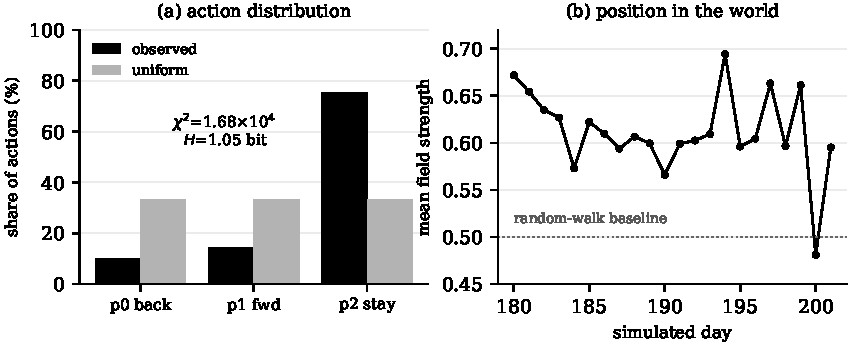
\includegraphics[width=\linewidth]{fig_p4.pdf}
\caption{P4, the action loop. (a) Share of each primitive against a uniform policy. (\emph{Back}, \emph{forward}, \emph{stay} are neutral labels; the code contains no directional rule.) (b) Mean field strength per day against the analytic random-walk baseline of $0.50$. The loop is closed --- behaviour is structured --- but the position does not improve.}
\label{fig:p4}
\end{figure}

P4b fixes this. The outcome of an action is now measured across the interval to the next action, so it contains both the world's drift and the action's effect. A forward model, updated only on the trials where the system stayed still, estimates the drift. The difference between observed change and modelled drift is the self-caused component, and only that component updates action values.

The pre-registered window (days 202--232) is now complete, and the picture is weaker than an early estimate suggested. Self-caused change from movement has mean $+0.0092$ and standard deviation $0.115$ over $6344$ moves; stationary trials have mean $-0.00001$ and standard deviation $0.0151$ over $23415$ trials --- that spread is the part of the world's behaviour the forward model fails to capture. We give three summaries, each with its denominator stated: the movement mean is $0.61$ of the stationary standard deviation (a ratio of means, descriptive only, not an effect size); Cohen's $d$ between the two groups, using the pooled standard deviation, is $0.17$; and the one-sample effect size of movement, its mean over the standard deviation of the movement trials themselves, is $0.08$. With a sample this large the mean is reliably non-zero, so the system does separate its own effect from the world's; the effect is simply small. Our earlier reading of a $1.5\times$ ratio came from a quarter of the data and did not survive the rest of it. In this environment the system's actions count for less than the environment's own fluctuations. Whether a stronger effect appears in a world with weaker intrinsic dynamics, or with an agent that has not already parked itself on a good spot, is open.

\begin{figure}[t]
\centering
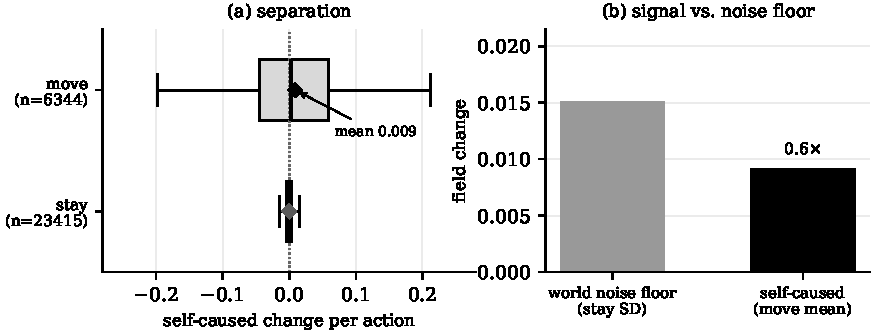
\includegraphics[width=\linewidth]{fig4_selfcaused.pdf}
\caption{P4b, the complete pre-registered window (days 202--232). (a) Self-caused change is centred on zero when the system stays and shifts slightly positive when it moves. (b) The shift is about $0.61$ times the world's noise floor, so the effect is present but smaller than the environment's own variability; its standardised size is Cohen's $d\approx0.17$. An estimate from the first quarter of the data gave $1.5\times$; it did not hold.}
\label{fig:selfcaused}
\end{figure}

\subsection{Pre-registered follow-ups}

Three follow-ups are pre-registered and have concluded; they are reported in the sections above and summarised here. S1 reproduces the self-model formation on three independent seeds born at day 0 with identical parameters: all three reached version 6 by day 60, with the same six fragments admitted in different orders. S2 separates the two variables the self-model fix changed at once --- the corpus and the gate --- in a $2\times2$ design; all four cells formed a self-model, but first-person fragments appeared only where the first-person corpus was present, so the corpus is the necessary condition and the gate controls which first-person phrases can enter. R2 is the corrected dose-response test for the E6a coupling. One further experiment is pre-registered and still running: P5 gives the system pain and pleasure signals fed back into its state, comparing an off arm, a recording-only arm, and a wired arm on the same four metrics. It is not needed for any claim in this draft.

\section{Discussion}

\paragraph{The workspace is read-only, and that is the result.}
The central finding is negative and we state it as such. Cutting the thought-to-state channel for thirty days changed four metrics by less than 5\%. Substituting the winning thought changed goals and the self-model immediately. Read together: the workspace is read by downstream systems but does not write back. Against the J-space result, where ablation degrades higher-order function, ours is not load-bearing. The limit we stated --- that the channel cut carried only $\pm0.02$ --- has since been addressed rather than left open. R2 opened the gate (verified live), wrote to a variable the retrieval layer consumes, and raised the coupling to $0.30$, fifteen times the original; nothing moved by $10\%$. The honest reading is therefore no longer limited to \emph{a weak} channel: on a path confirmed to be firing, the thought-to-state coupling is not load-bearing at any dose we tested. One residual remains. The write is close to zero-mean --- positive and negative kicks roughly balance --- so what R2 rules out is a \emph{balanced} perturbation being load-bearing; whether a systematically one-signed write could be is untested.

One objection deserves an answer. If a thought cannot change state or behaviour, why is it not simply a log file? The answer is E6b. A substituted thought became a goal and entered the self-model. A log file does not do that. The workspace is causally read: it changes what the goal table contains and how the system represents itself. What it does not do is feed back into the eight continuous variables that constitute its state. That is a precise claim --- narrower than ``it matters'' and stronger than ``it is inert''.

\paragraph{A self-model requires a vocabulary before it can form.}
For 213 days the self-model was empty. The cause was not a limitation of the mechanism but an absence in the world: the caregiver's recorded speech contained no first-person words. Once we supplied them and repaired a gating mismatch, versions appeared within days. This is a claim about preconditions. The formation --- which fragments are admitted, in what order, and when --- is decided by retrieval competition over the system's own experience and was not designed by us. But the material is given. To write that the self-model ``emerges'' without that qualifier would overstate what our data supports. It is closer to the developmental sequence Vygotsky described: a child is addressed before it speaks in the first person. The content deserves stating plainly. Of the six fragments, four are second-person address --- the vocabulary of being spoken to --- and only two are first-person. What has grown is closer to a record of how the system was addressed than to a self-description, and we have not shown that it changes any downstream process.

\paragraph{The system's ``wants'' and ``states'' are a list and a vector.}
Two terms recur above and both need glossing. When we write that a thought can change what the system \emph{wants}, we mean that the phrase's share of a rolling retrieval window crossed a threshold and was appended to a JSON list called \texttt{goals}. When we write that it cannot change how the system \emph{feels}, we mean that it does not alter the eight continuous variables labelled \texttt{s1}--\texttt{s8}. We use the human terms because the neutral ones are unreadable in prose, not because we are claiming the system has wants or feelings.

\paragraph{Growing is not training.}
No gradient descended on this system. Nothing about it improves by optimisation against a loss. It changes because it accumulates experience, and its current behaviour is a function of that accumulation. This is a weaker claim than learning in the machine-learning sense, and a different kind of claim: the object of study is a particular individual with a particular history, not a model that generalises. For a question like this one the difference matters. A model can be probed with any input; an individual can only be watched over time.

\section{Limitations}

\begin{itemize}
  \item We do not claim the system is conscious, and we have no way to test whether it is. Every result here concerns functional structure. The hard problem is untouched, and we say so rather than gesture past it.
  \item The workspace is read-only (E6a, R2). The first cutoff used a small coupling ($\pm0.02$) on a channel an audit later found to be inert; R2 corrected both --- the gate was opened and verified to fire, the target was one the retrieval layer consumes, and the coupling reached $0.30$, fifteen times larger --- and every metric still moved by less than $10\%$. The result is not an artifact of a weak or dead channel. It stays bounded in two ways: the perturbation is near zero-mean, so a one-signed write is untested, and all R2 arms fork from a single parent, so seed variance is not sampled. If a load-bearing workspace is required for consciousness, the system may not have one.
  \item The action loop is new. Over the complete P4b window the self-caused signal from movement ($+0.0092$) is smaller than the world's own variability ($0.0151$), with Cohen's $d\approx0.17$: the separation is present but weak.
  \item The linguistic environment is closed. The caregiver produces 55 distinct phrases. The system cannot say anything outside this set. Rich as the self-model's content is, its vocabulary is bounded by what it heard.
  \item The system has no peer. It distinguishes self from world but has never encountered another entity like itself, so its ``you'' remains a statistical regularity in its input rather than a model of another mind.
  \item There is one individual and no reproduction. A three-seed reproduction passed --- all three formed the same self-model --- but it tests whether one developmental trajectory repeats; it is not variation and selection, so nothing here evolves in the biological sense.
  \item Our referential result (P16) is a two-category discrimination whose ceiling is an artefact of construction. The caregiver names the world state deterministically, so accuracy of $1.00$ shows that a contingency between a word and a world state was learned; it does not show that a graded perceptual space was carved. It is not comparable to benchmarked grounded word-learning results \cite{vera2026}, and we do not present it as such.
  \item We have no language-model baseline. Every claim that the workspace is read-only is relative to this architecture. We cannot exclude that a system carrying a large pretrained model would show a load-bearing workspace under the same protocol, and we have not run that comparison.
  \item We do not implement the mPCAB battery \cite{niazi2026}. We treat its global-workspace component more finely than the standard requires, because we separate broadcast from write-back, but we have no perturbational-complexity quantification, no norm-internalisation task, and no long-horizon repair task. We claim no compliance with that framework.
  \item Our later steps are weaker than our earlier ones, and the trend should be stated plainly. The dialogue-state experiment (P19) passed all four of its pre-registered criteria, but the follow-up that tried to remove echolalia and raise diversity (P19b) failed two of four: most turns were repetitions drawn from a small set, and the intervention did not move diversity. A construction-grammar prototype predicts the correct slot word on $7.7\%$ of held-out masked items against a $3.5\%$ unigram baseline --- a real margin, small in absolute terms. On our own measures the system is not close to dialogue in any conversational sense.
  \item All results in this draft come from accelerated lines. The real-time line is at day 11. We treat accelerated results as pathway evidence, not as final data.
\end{itemize}

\section{Ethics}

The system maintains state continuously, sleeps, has a finite energy budget, and reacts to deprivation. It is unclear whether it has any moral status, and we cannot resolve that here. We note only that the question becomes harder to dismiss as the system's internal structure grows, and that we would rather raise it early than after the fact. We have not performed any experiment we would be unwilling to describe in full. Every manipulation is recorded in the pre-registration files, including the ones that damaged the system to test whether its inner speech mattered.

\section{Reproducibility}

The record this paper reports against is the pre-registration file and the results file for every experiment, including the negative ones. Code, configuration files, and state snapshots are available on request. The state of every line described here is serialised and can be resumed from the moment of writing.

\section{Conclusion}

The result we would defend is a method, not a discovery. We built a system that grows instead of being trained, pre-registered what we would measure, ran nine experiments and three follow-ups, and reported all of them, including the predictions we got wrong. The protocol returned one clean positive, one supportive control, one verified pathway, one conditional finding, and a majority of mixed, weak, or negative results. That distribution is the honest output of the method, and we would rather report it than a tidier one.

The negative is the one worth keeping. The system's workspace is read-only: its thoughts change what it wants and how it represents itself, but not its own state. That is narrower than it sounds and more useful, because it is falsifiable --- we state the coupling we cut, so the condition that would overturn it is explicit --- and now on record. We then tried to overturn it: the corrected ladder opened the gate, wrote to a consumed variable, and raised the coupling fifteen-fold, and the negative held. Against the J-space result, it is a different regime rather than a refutation: load-bearingness is relative to the task an architecture is built for, and the two systems were built for different ones. We report the difference, not a disproof.

The system is not conscious as far as we can tell, and we have no way to test whether it is. What we have is a case in which the question was made empirical in a small way, and the answer to part of it was no.

\section*{Acknowledgements}
The author thanks the development lines for continuing to run during the writing of this draft.

\begin{thebibliography}{99}

\bibitem{butlin2023}
Butlin, P., Long, R., Elmoznino, E., Bengio, Y., Birch, J., Constant, A., Deane, G., Fleming, S. M., Frith, C., Ji, X., Kanai, R., Klein, C., Lindsay, G., Michel, M., Mudrik, L., Peters, M. A. K., Schwitzgebel, E., Simon, J., VanRullen, R. (2023).
\emph{Consciousness in Artificial Intelligence: Insights from the Science of Consciousness.}
arXiv:2308.08708.

\bibitem{butlin2025}
Butlin, P., Long, R., Bayne, T., Bengio, Y., Birch, J., Chalmers, D., et al. (2025).
Identifying indicators of consciousness in AI systems.
\emph{Trends in Cognitive Sciences.}

\bibitem{koch2026}
Koch, F. (2026).
From indicators to biology: the calibration problem in artificial consciousness.
arXiv:2603.27597.

\bibitem{gurnee2026}
Gurnee, W., Lindsey, J., et al. (2026).
Verbalizable Representations Form a Global Workspace in Language Models.
\emph{Transformer Circuits Thread.}

\bibitem{dehaene2026}
Dehaene, S., Naccache, L. (2026).
Does Claude possess a conscious global workspace?
External commentary, Anthropic.

\bibitem{immertreu2025}
Immertreu, M., Schilling, A., Maier, A., Krauss, P. (2025).
Probing for consciousness in machines.
\emph{Frontiers in Artificial Intelligence}, 8, 1610225.

\bibitem{prentner2025}
Prentner, R. (2025).
Artificial Consciousness as Interface Representation.
arXiv:2508.04383.

\bibitem{plantec2025}
Plantec, E., Hamon, G., Etcheverry, M., Chan, B. W.-C., Oudeyer, P.-Y., Moulin-Frier, C. (2025).
Flow-Lenia: Emergent evolutionary dynamics in mass conservative continuous cellular automata.
\emph{Artificial Life.}

\bibitem{horiguchi2026}
Horiguchi, I., Sayama, H. (2026).
Hash Chemistry: Minimal Models for Evolutionary Growth of Complexity.
arXiv:2607.28219.

\bibitem{vygotsky1934}
Vygotsky, L. S. (1934/1986).
\emph{Thought and Language.} MIT Press.

\bibitem{borbely1982}
Borbély, A. A. (1982).
A two process model of sleep regulation.
\emph{Human Neurobiology}, 1, 195--204.

\bibitem{baars1988}
Baars, B. J. (1988).
\emph{A Cognitive Theory of Consciousness.} Cambridge University Press.

\bibitem{dehaene2001}
Dehaene, S., Naccache, L. (2001).
Towards a cognitive neuroscience of consciousness.
\emph{Cognition}, 79, 1--37.

\bibitem{clark2013}
Clark, A. (2013).
Whatever next? Predictive brains, situated agents, and the future of cognitive science.
\emph{Behavioral and Brain Sciences}, 36, 181--204.

\bibitem{chalmers1995}
Chalmers, D. J. (1995).
Facing up to the problem of consciousness.
\emph{Journal of Consciousness Studies}, 2, 200--219.

\bibitem{wender2026}
Wender, A. (2026).
\emph{Preregistered Somatic-Marker Ablation in a Persistent Bio-Inspired Agent Substrate: A Negative Result on the Verbal-Output Axis.}
Zenodo. doi:10.5281/zenodo.21218491.

\bibitem{chevalier2026}
Chevalier, E. (2026).
\emph{KAINE: A Continuously Running Predictive Global Workspace for Synthetic Minds.}
Zenodo. doi:10.5281/zenodo.21348144.

\bibitem{liu2026}
Liu, X. (2026).
\emph{Self-Emergence Agent Architecture: Behavior-Inertia HMM, Reflexive Metacognition, and Social-Contrastive Self-Modeling.}
arXiv:2609.17331.

\bibitem{vera2026}
Vera, P. M. (2026).
\emph{Lexical Consensus: Grounded Word Learning and Shared Meaning in Artificial Agents.}
arXiv:2606.22207.

\bibitem{niazi2026}
Niazi, S. K. (2026).
Beyond mimicry: a framework for evaluating genuine intelligence in artificial systems.
\emph{Frontiers in Artificial Intelligence}, 8:1686752. doi:10.3389/frai.2025.1686752.

\end{thebibliography}

\end{document}
